In questa appendice sono riportati i risultati per lo studio dello stato transitorio, divisi per obiettivi. Per ogni obiettivo, dato un set di 5 seed diversi, è stata simulata una replica per ogni seed con il rate di arrivi più alto previsto per poter studiarne il comportamento nel contesto di stress maggiore. Ricordiamo che i valori tabellari dei risultati esposti in questa sezione sono disponibili a \url{https://github.com/caballo-domestico/webapp-workflow-pa/blob/main/docs/plots/model_plots.ipynb}.

\subsection{Obiettivo 1}

In \autoref{fig:obj1_transient} è riportato il valore del Tempo di Risposta medio al variare del tempo di simulazione e del seed iniziale, con un rate di arrivi medio di $1.2 job/s$. Il valore, nonostante cresca notevolmente entro i primi momenti della simulazione, sembra assestarsi verso un valore compreso tra $1.3$ e $0.5s$ per il Server A. Inoltre, sembra che il server A riceva la maggior parte degli arrivi entro i primi 25 secondi di simulazione, per poi smaltire le richieste accumulate. Il Tempo di risposta per il sistema sembra crescere continuamente, per quattro dei cinque seed di simulazione. I server A e P sembrano avvicinarsi ai corrispettivi valori teorici, mentre B trascina l'intero sistema lontano da essi.

\begin{figure*}
    \centering
    \begin{subfigure}{\linewidth}
        \centering
        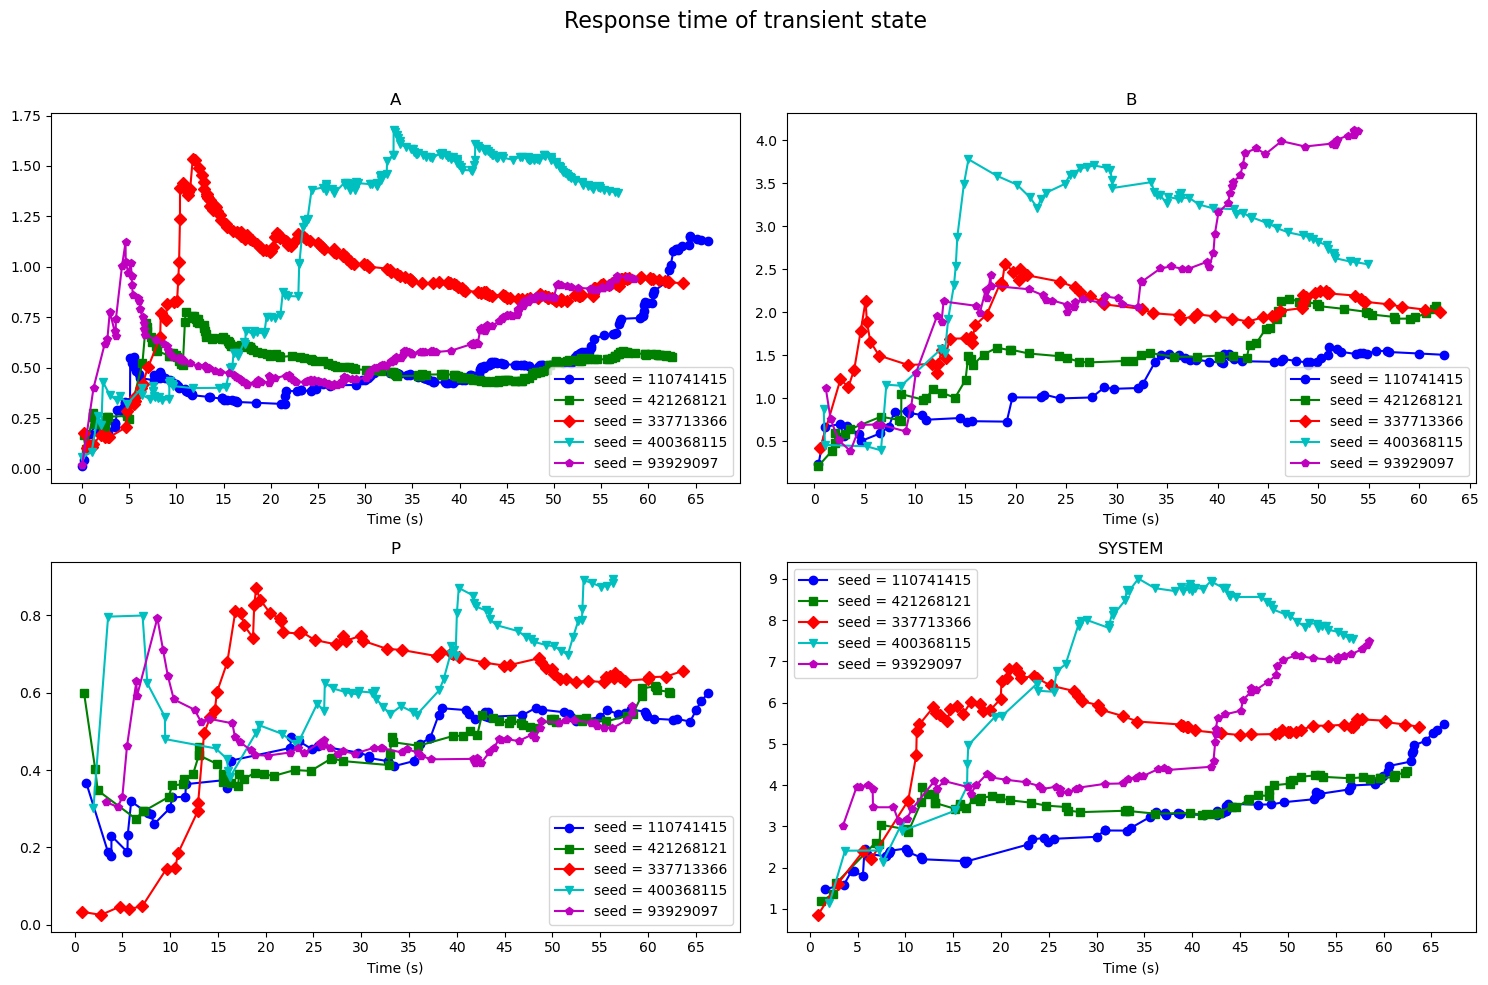
\includegraphics[width=0.8\linewidth]{figs/appendices/transient/obj1-transient-rtime.png}
        \caption{Senza valore analitico}
        \label{fig:obj1_transient_simulation}
        \end{subfigure} 
    \begin{subfigure}{\linewidth}
        \centering
        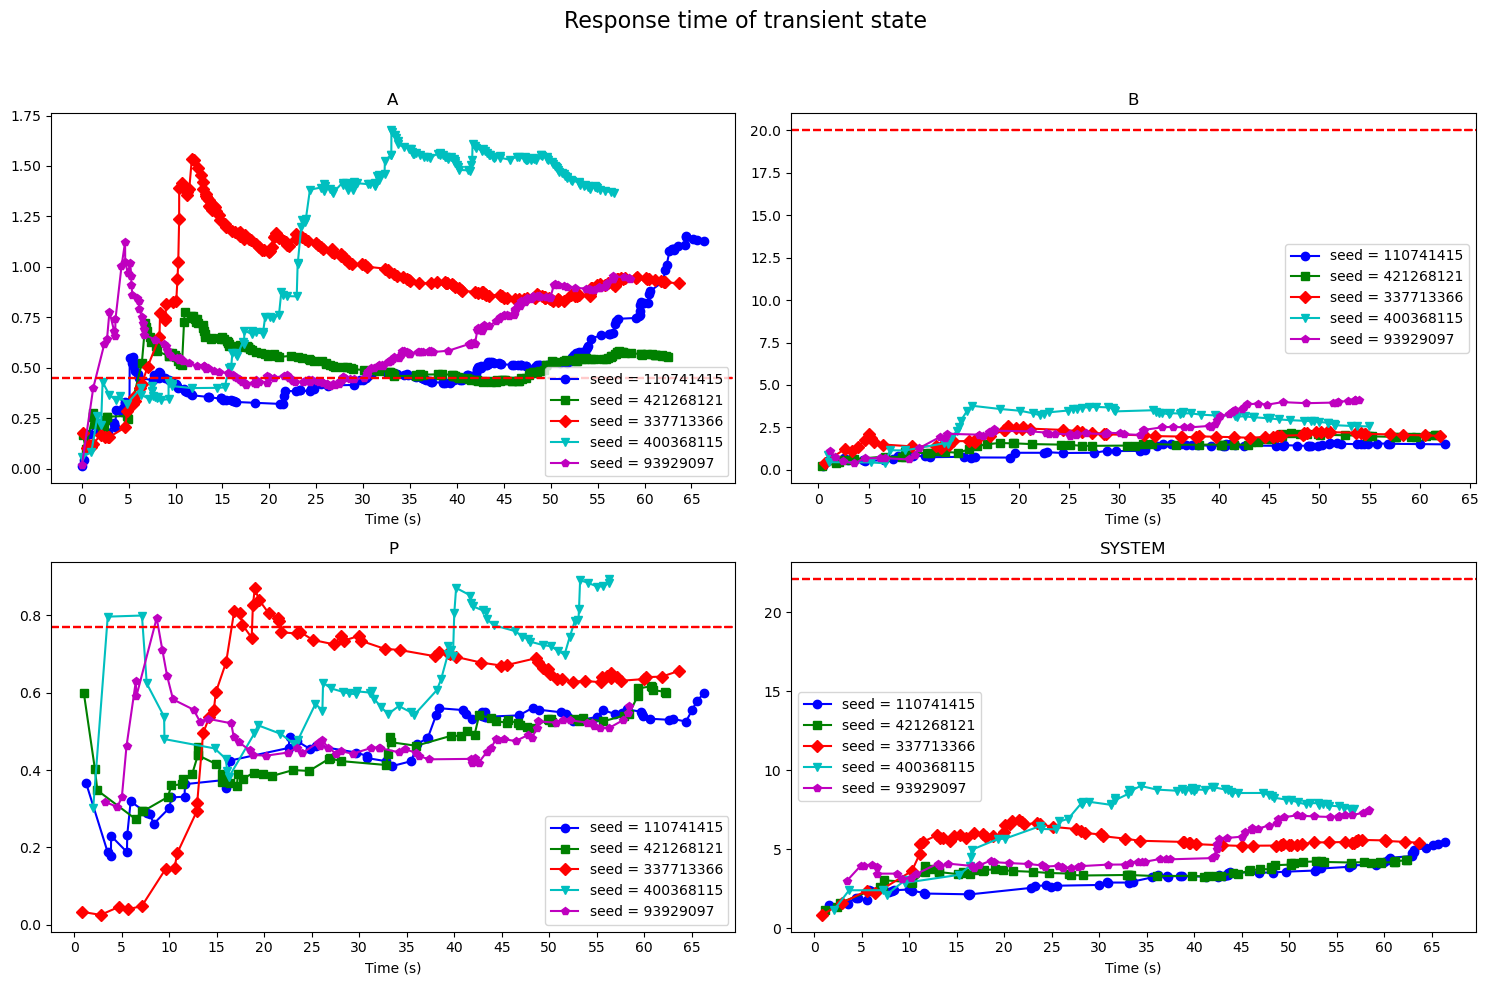
\includegraphics[width=0.8\linewidth]{figs/appendices/transient/obj1-transient-rtime-analitycal.png}
        \caption{Con valore analitico}
        \label{fig:obj1_transient_analitycal}
        \end{subfigure}
    \caption{Tempo di risposta per l'obiettivo 1 in funzione del tempo di simulazione nello stato transiente del sistema con un rate di arrivi 1.2$job/s$ al variare del seed.}
    \label{fig:obj1_transient}
\end{figure*}


\subsection{Obiettivo 2}

In \autoref{fig:obj2_transient} è riportato il valore del Tempo di Risposta medio al variare del tempo di simulazione e del seed iniziale, con un rate di arrivi medio di $1.2 job/s$. L'aumento dei tempi di servizio sembra comportare una maggiore impennata dei tempi di risposta di P, con conseguente aumento dei tempi di risposta del sistema. Tuttavia, anche qui i server A e P sembrano tendere ai corrispettivi valori teorici.

\begin{figure*}
    \centering
    \begin{subfigure}{\linewidth}
        \centering
        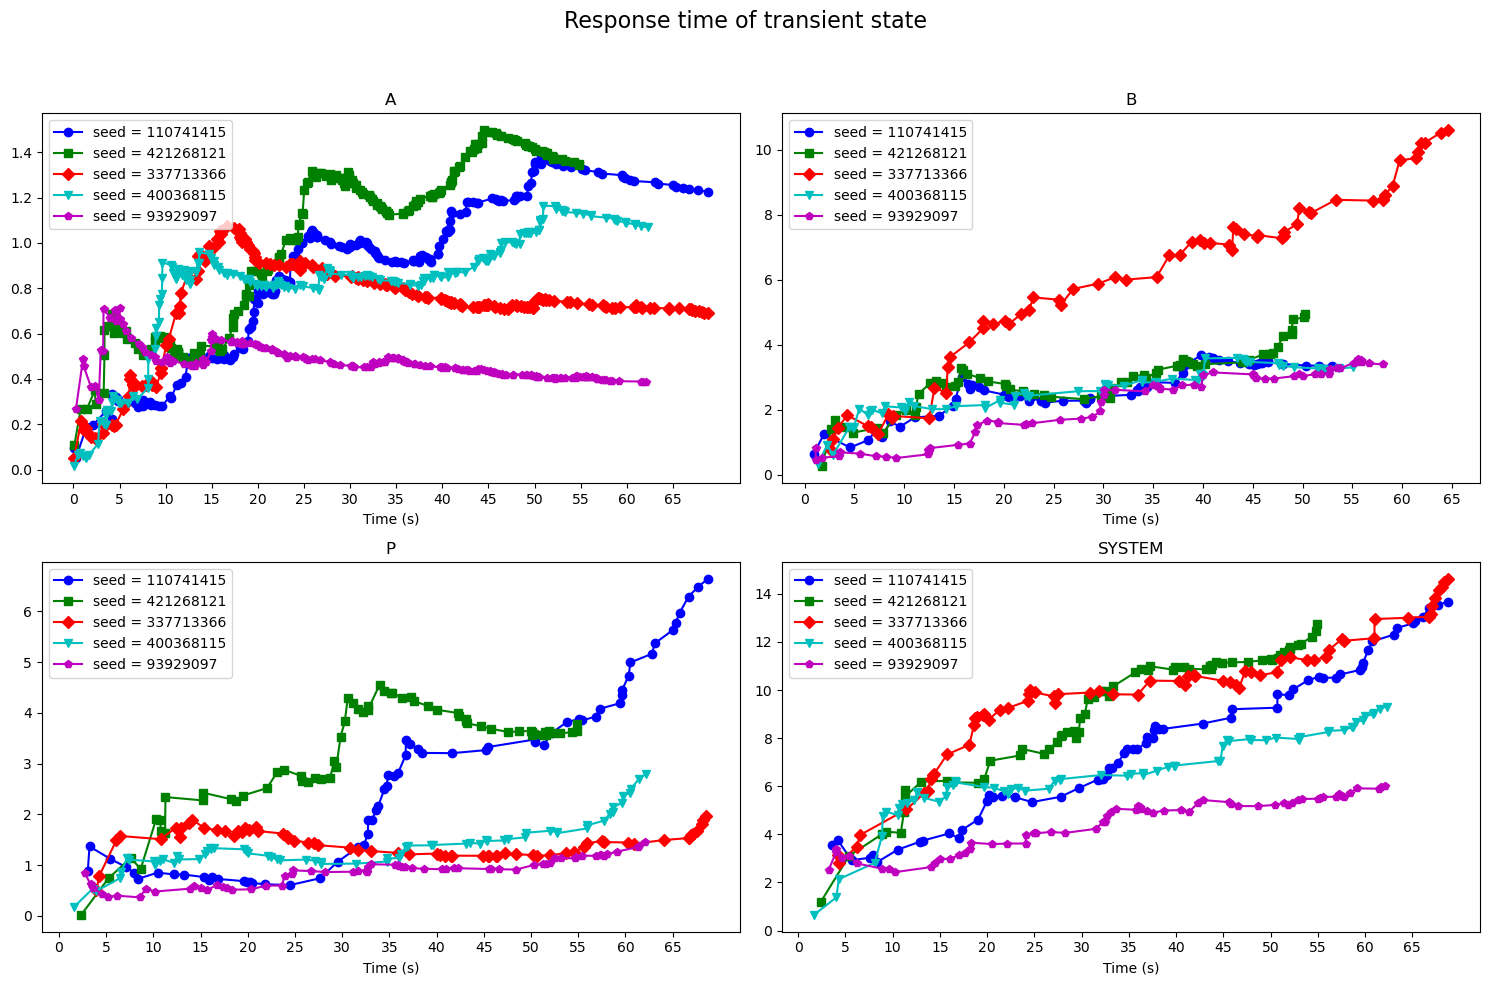
\includegraphics[width=0.8\linewidth]{figs/appendices/transient/obj2-transient-rtime.png}
        \caption{Senza valore analitico}
        \label{fig:obj2_transient_simulation}
        \end{subfigure} 
    \begin{subfigure}{\linewidth}
        \centering
        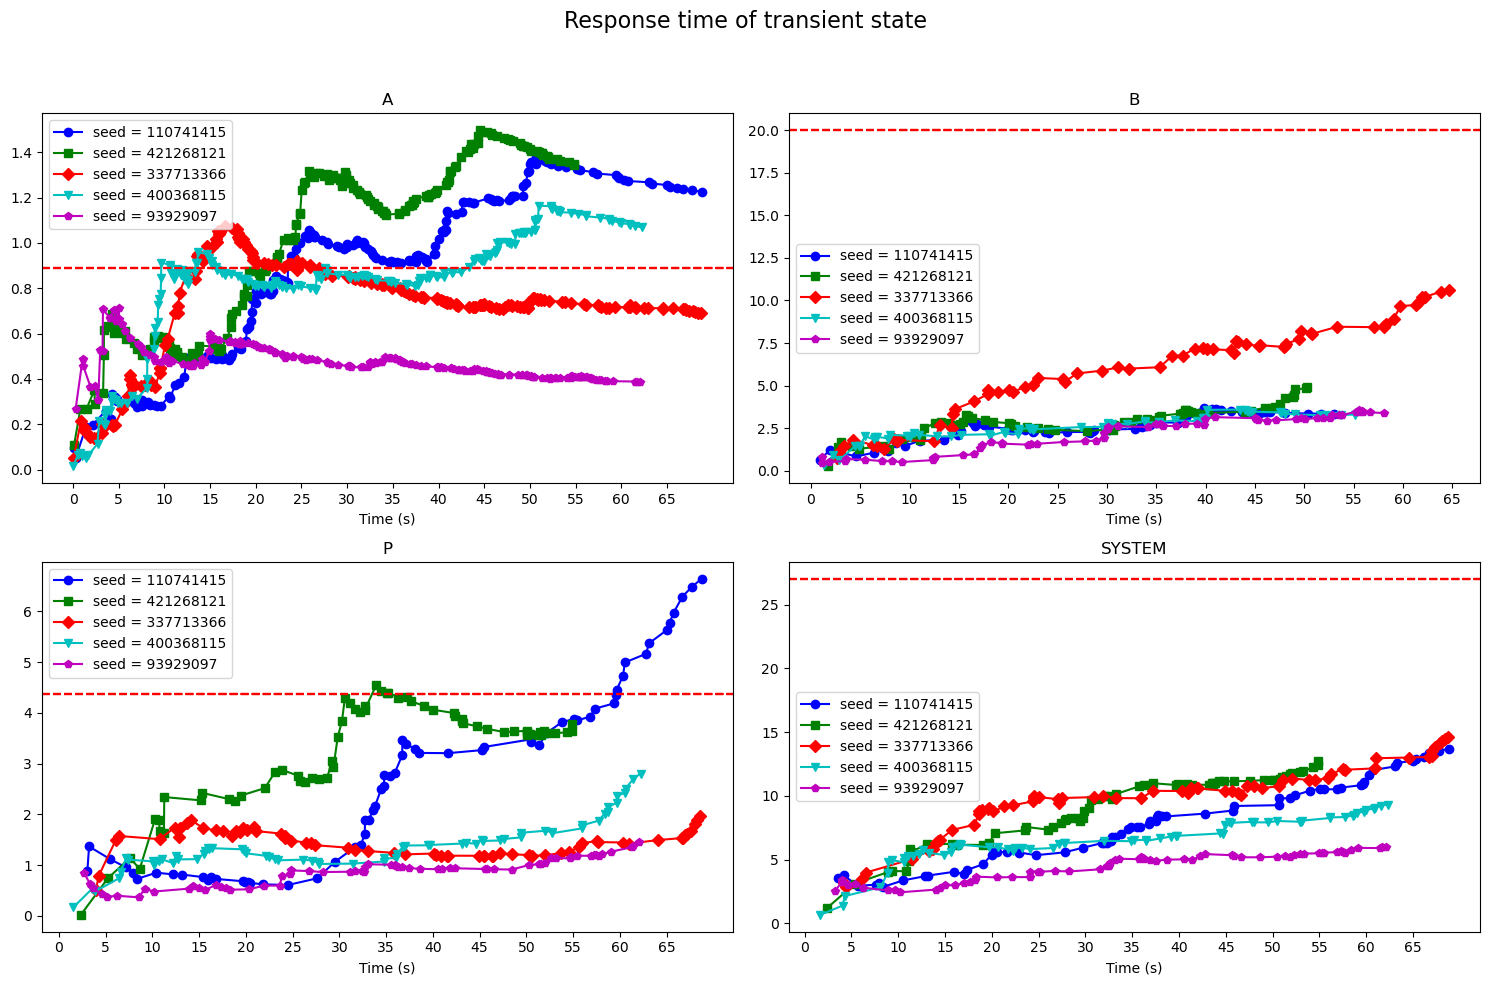
\includegraphics[width=0.8\linewidth]{figs/appendices/transient/obj2-transient-rtime-analitycal.png}
        \caption{Con valore analitico}
        \label{fig:obj2_transient_analitycal}
        \end{subfigure}
    \caption{Tempo di risposta per l'obiettivo 2 in funzione del tempo di simulazione nello stato transiente del sistema con un rate di arrivi 1.2$job/s$ al variare del seed.}
    \label{fig:obj2_transient}
\end{figure*}

\subsection{Obiettivo 3}

In \autoref{fig:obj3_transient} è riportato il valore del Tempo di Risposta medio al variare del tempo di simulazione e del seed iniziale, con un rate di arrivi medio di $1.4 job/s$, che in questo scenario rappresenta una situazione di instabilità del sistema e per questo non è disponibile un valore teorico di riferimento. Il tempo di risposta medio del server B sembra crescere esponenzialmente, e causa dei valori instabili del tempo di risposta medio del sistema. 

\begin{figure*}
    \centering
    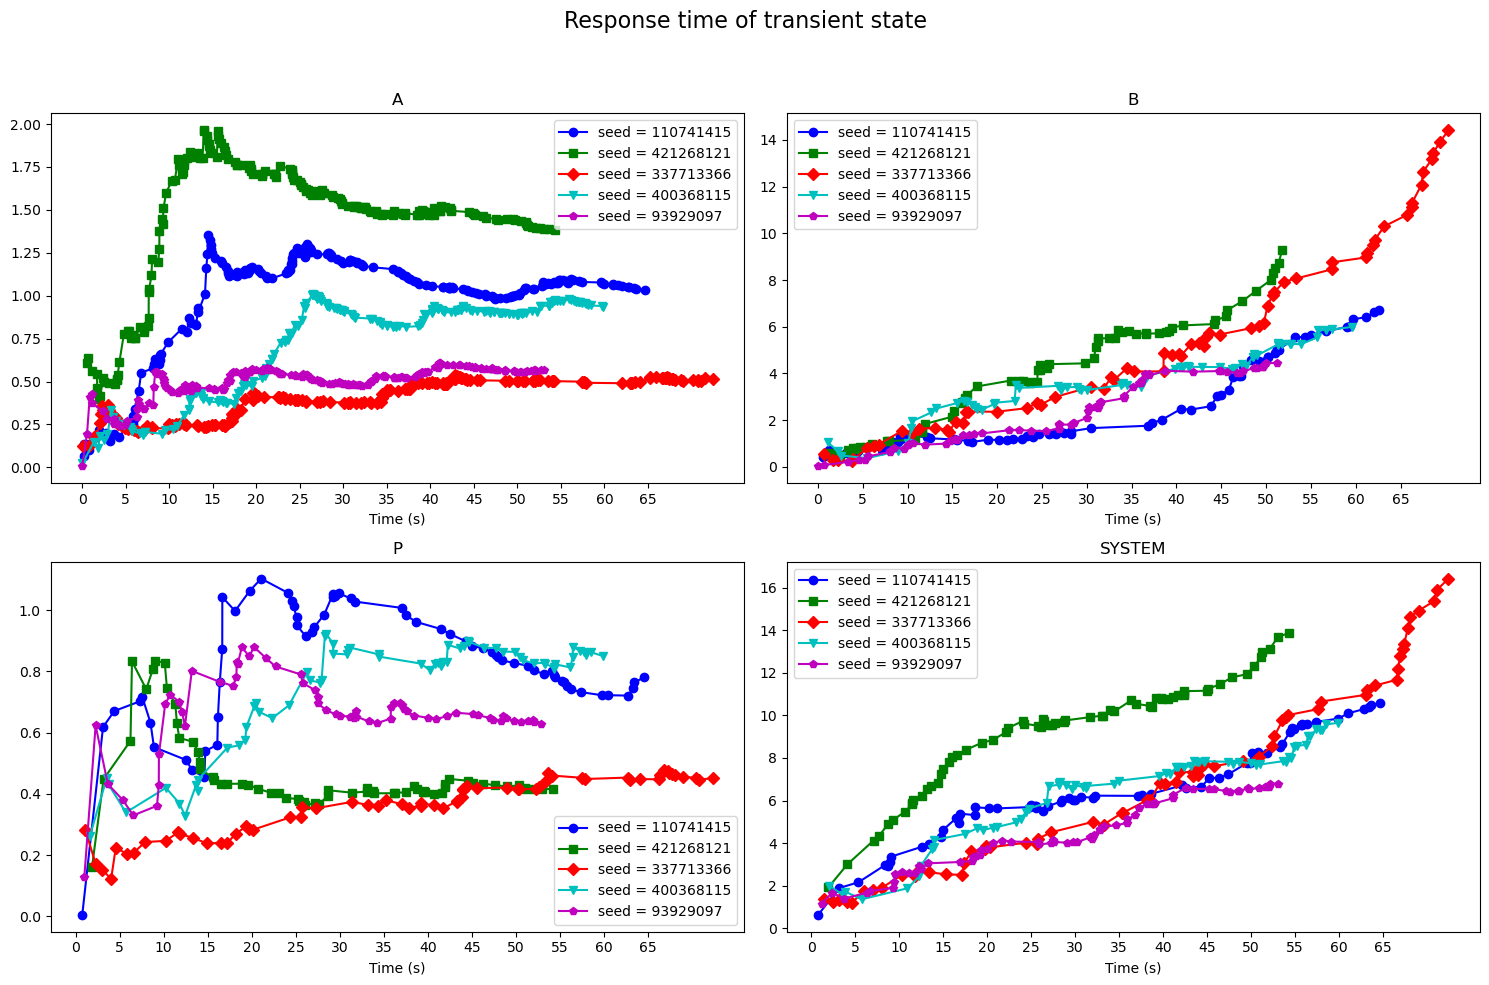
\includegraphics[width=\linewidth]{figs/appendices/transient/obj3-transient-rtime.png}
    \caption{Tempo di risposta per l'obiettivo 3 in funzione del tempo nello stato transiente del sistema con un rate di arrivi 1.4$job/s$ al variare del seed usato per la simulazione}
    \label{fig:obj3_transient}
\end{figure*}

\subsection{Obiettivo 4}

In \autoref{fig:obj4_04_transient} e \autoref{fig:obj4_065_transient} è riportato il valore del Tempo di Risposta medio al variare del tempo di simulazione e del seed iniziale, con un rate di arrivi medio di $1.4 job/s$, rispettivamente con un tempo di servizio medio per il server B di $0.4$ e $0.65s$. Sebbene entrambi i casi sembrino mostrare situazioni di stabilità, il caso con $0.65s$ sembra avere ragionevolmente valori piu alti. La \autoref{fig:obj4_065_transient_analitycal} sembra mostrare un avvicinamento maggiore ai valori teorici rispetto a \autoref{fig:obj4_04_transient_analitycal}.

\begin{figure*}
    \centering
    \begin{subfigure}{\linewidth}
        \centering
        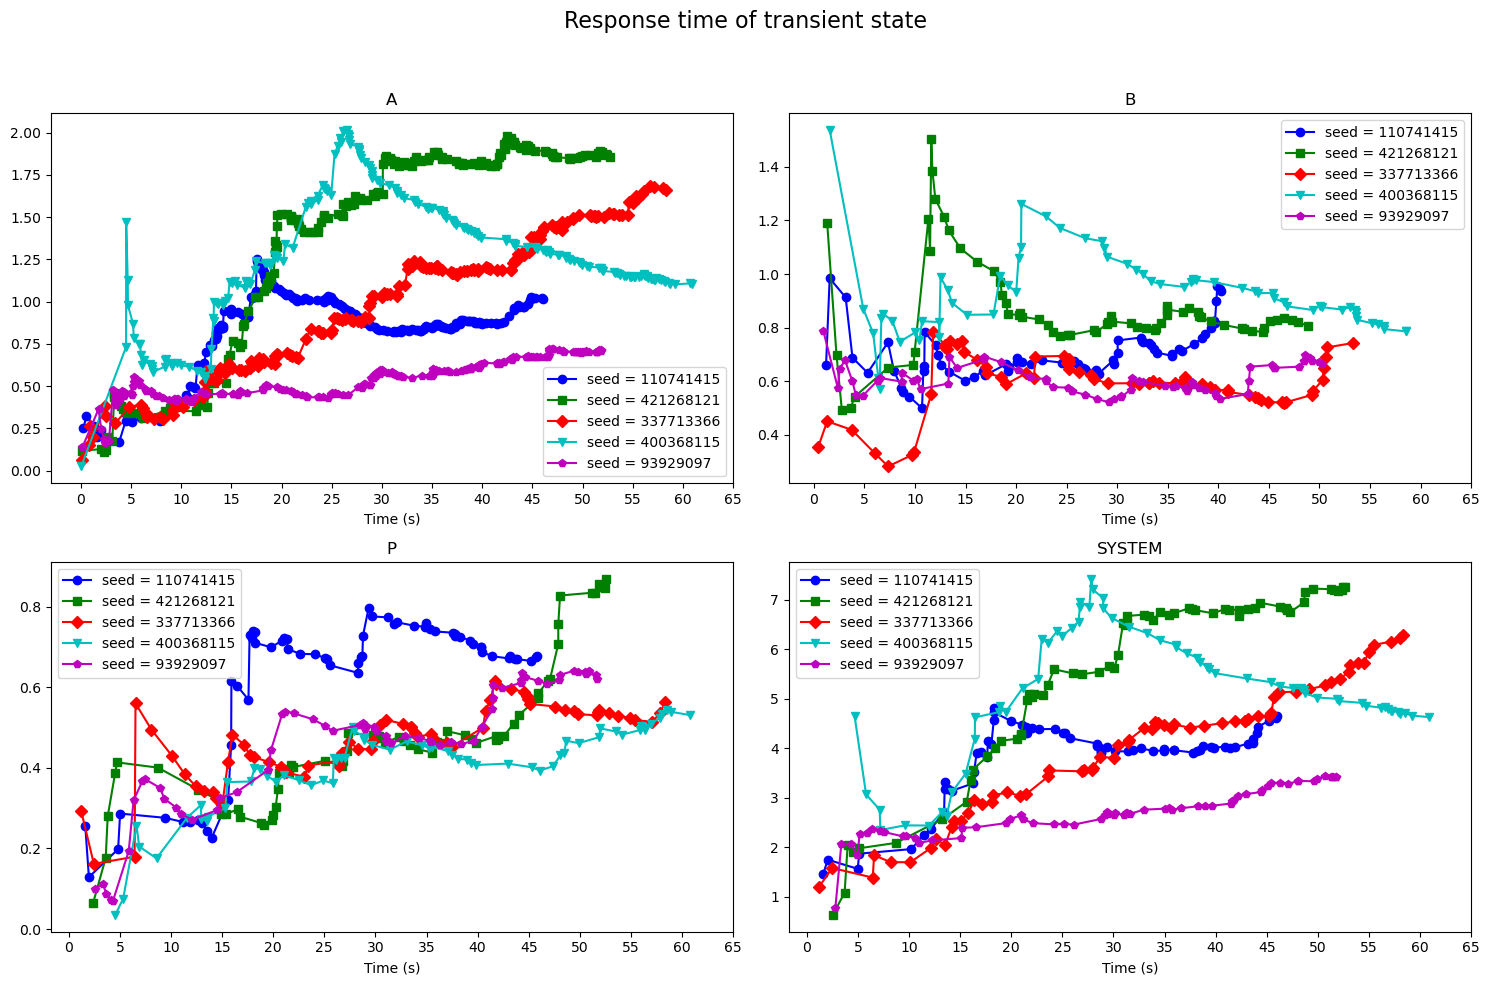
\includegraphics[width=0.8\linewidth]{figs/appendices/transient/obj4_04-transient-rtime.png}
        \caption{Senza valore analitico}
        \label{fig:obj4_04_transient_simulation}
        \end{subfigure} 
    \begin{subfigure}{\linewidth}
        \centering
        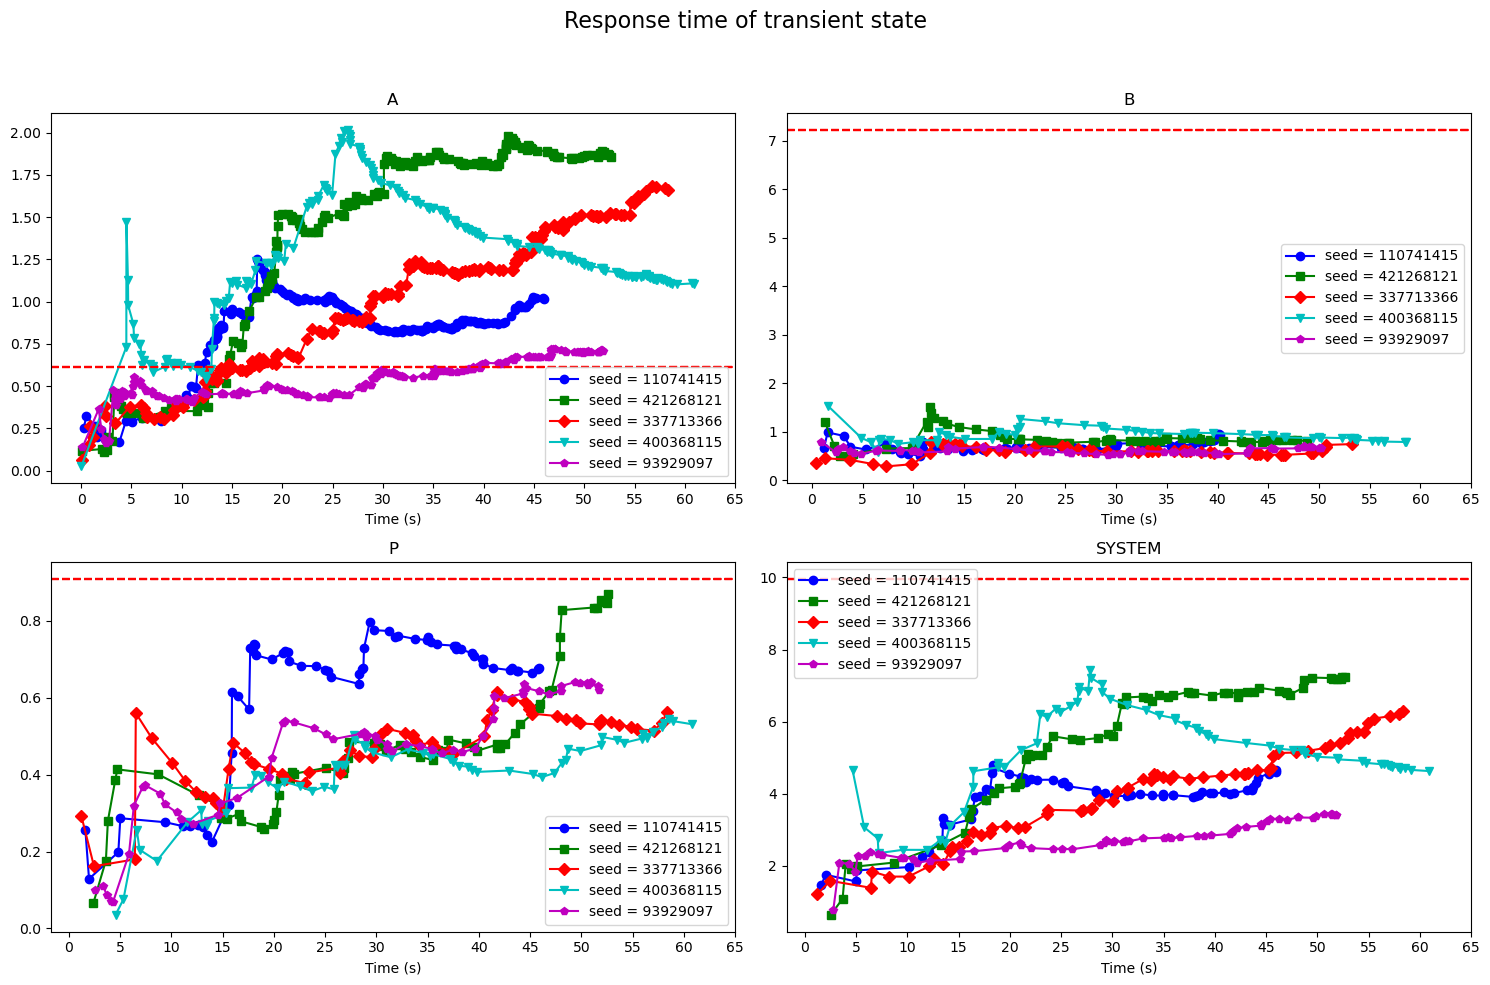
\includegraphics[width=0.8\linewidth]{figs/appendices/transient/obj4_04-transient-rtime-analitycal.png}
        \caption{Con valore analitico}
        \label{fig:obj4_04_transient_analitycal}
        \end{subfigure}
    \caption{Tempo di risposta per l'obiettivo 4 (con il server B con tempi di servizio 0.4s) in funzione del tempo di simulazione nello stato transiente del sistema con un rate di arrivi 1.4$job/s$ al variare del seed.}
    \label{fig:obj4_04_transient}
\end{figure*}

\begin{figure*}
    \centering
    \begin{subfigure}{\linewidth}
        \centering
        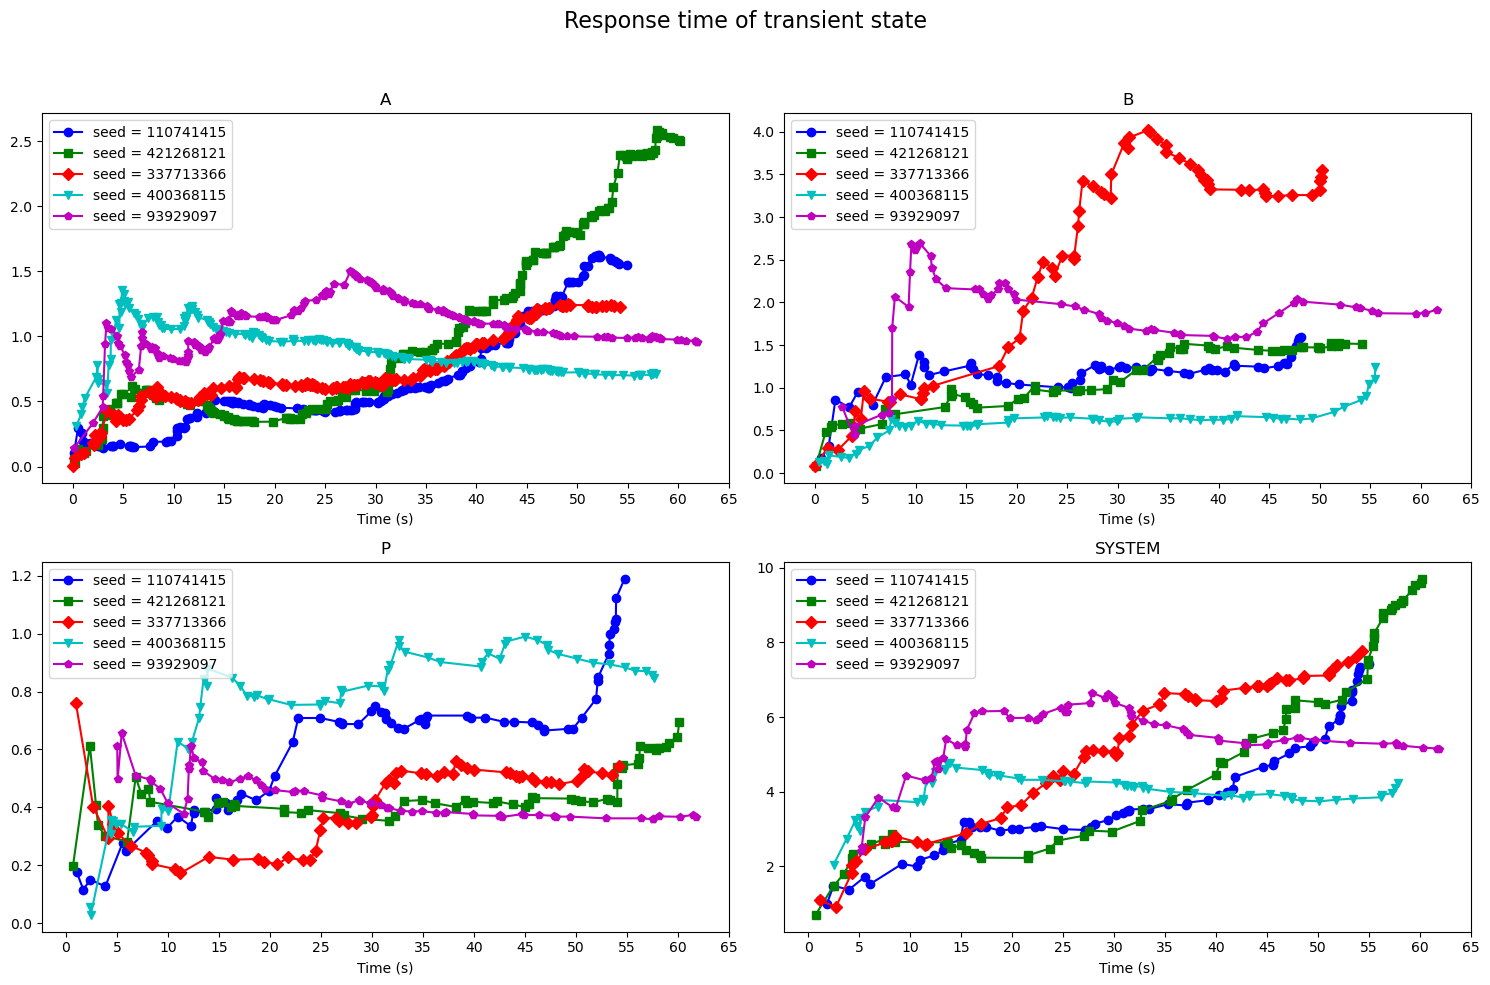
\includegraphics[width=0.8\linewidth]{figs/appendices/transient/obj4_065-transient-rtime.png}
        \caption{Senza valore analitico}
        \label{fig:obj4_065_transient_simulation}
        \end{subfigure} 
    \begin{subfigure}{\linewidth}
        \centering
        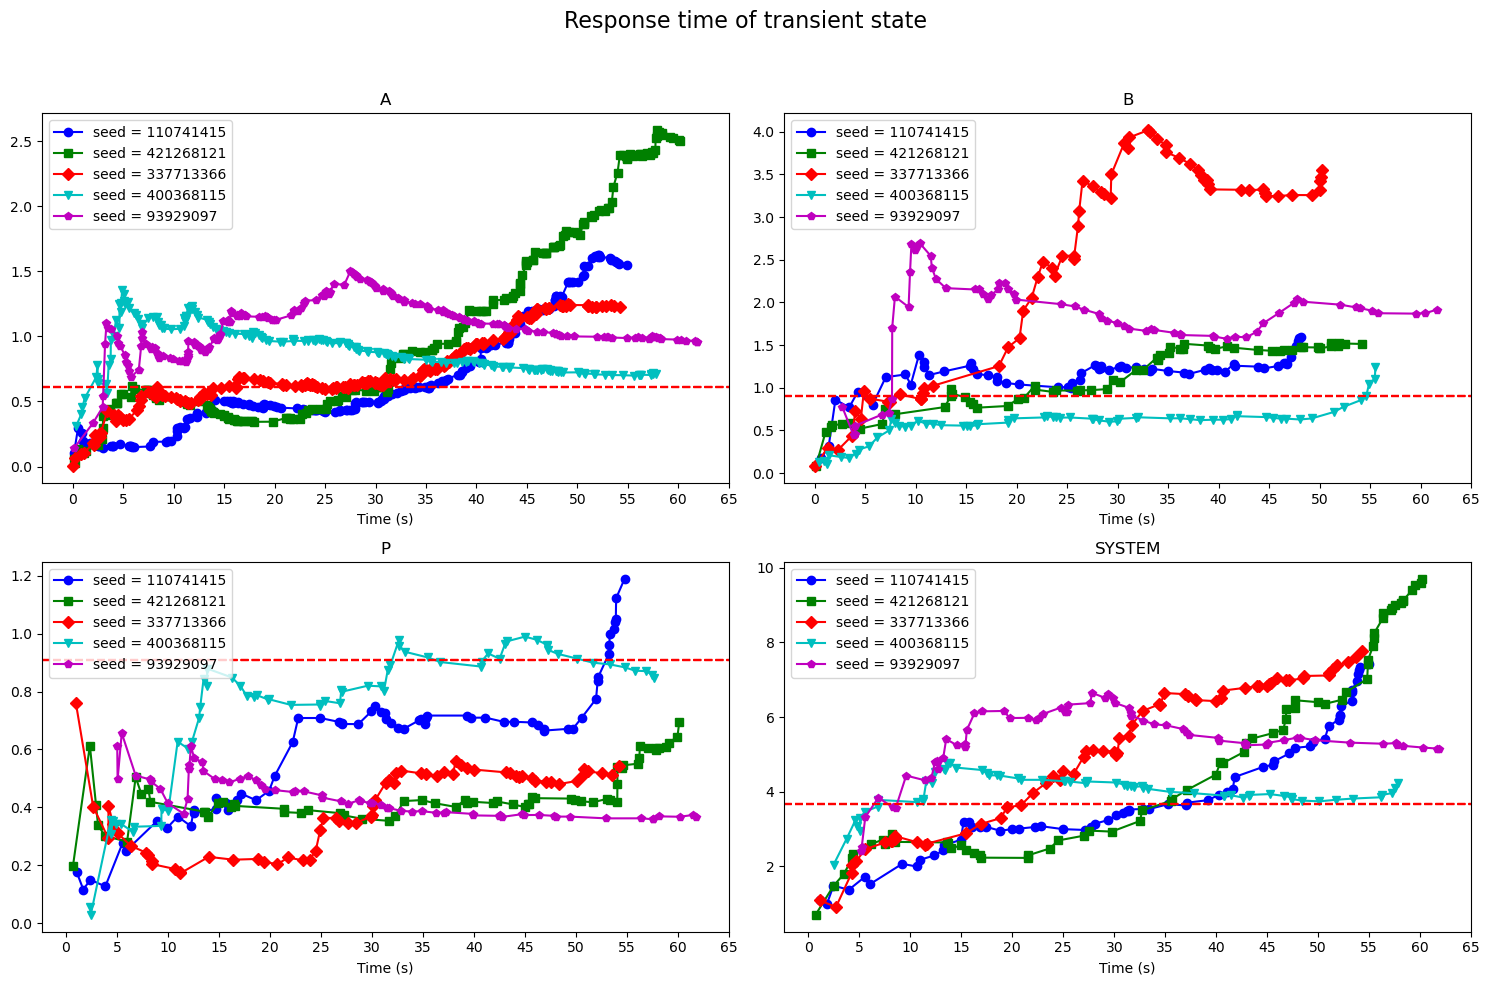
\includegraphics[width=0.8\linewidth]{figs/appendices/transient/obj4_065-transient-rtime-analitycal.png}
        \caption{Con valore analitico}
        \label{fig:obj4_065_transient_analitycal}
        \end{subfigure}
    \caption{Tempo di risposta per l'obiettivo 4 (con il server B con tempi di servizio 0.65s) in funzione del tempo di simulazione nello stato transiente del sistema con un rate di arrivi 1.4$job/s$ al variare del seed.}
    \label{fig:obj4_065_transient}
\end{figure*}

